% Chapter 1

\chapter{Introduction} % Main chapter title

\label{Chapter1} % Change X to a consecutive number; for referencing this chapter elsewhere, use \ref{ChapterX}

The internet is constantly growing and new network sevices arise constantly. This has as effect that security flaws become more and more important. Considering this, it becomes more important to be able to detect and prevent attacks on network systems.

\section{Intrusion detection systems}
An intrusion detection system is a system which tries to determine whether a system is under attack, to detect intrusions within a system. There are different types of intrusion detection systems or IDS. There are network-based intrusion detection systems and host-based intrusion detection systems. This thesis will uses machine learning techniques to detect malicious network behaviour, as such only network-based intrusion detection systems are covered.
\begin{figure}[H]
\centering
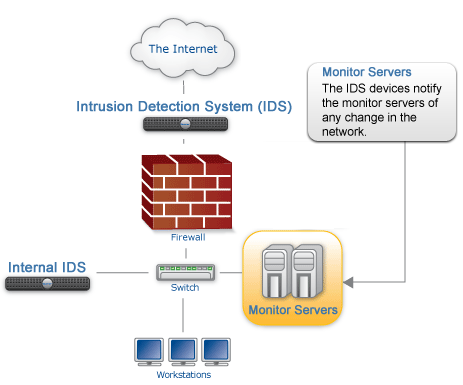
\includegraphics[width=0.6\textwidth]{Figures/idsdiagram}
\decoRule
\caption[Possible placement of IDS]{An IDS can for example be placed within the network or just before the network.}
\label{fig:IDS}
\end{figure}
\subsection{Host-based Intrusion Detection Systems}
Host-based intrusion detection systems are systems that monitor the device on which they are installed. The way they monitor the system can range from monitoring the state of the main system through log files, to monitoring program execution. In this way they can be quite indistinguishable from Anti-Virus programs.

\subsection{Network-based Intrusion Detection Systems}
Network-based intrusion detection systems are placed at certain points within a network in order to monitor traffic from and to devices within the network. The system can analyse the traffic using multiple techniques to determine whether the data is malicious. There are two different ways to analyse the network data. The analysis can be packet-based or flow-based.\\
\\
Packet-based analysis uses the entire packet including the headers and payload. An intrusion detection system that uses packet-based analysis is called a packet-based network intrusion detection system. The advantage of this type of analysis is that there is a lot of data to work with. Every single byte of the packet could be used to determine whether the packet is malicious or not. The disadvantage is immediately obvious once we look at networks through which a lot of data passes, such as data centers. Analysing every byte is very work-intensive and near impossible to do in such environments. \cite{alaidaros2011overview} \\
\\
Flow-based analysis doesn't use individual packets but uses general data about network flows. An intrusion detection system that uses flow-based analysis is called a flow-based network intrusion detection system. A flow is defined as a single connection between the host and another device. A flow can be defined using a (source\_IP, destination\_IP, source\_port, destination\_port) tuple. However flowdata also contains other information such as the duration of the connection, the start time, the amount of bytes and/or packets within the flow. Flow data can even contain data such as the amount of SYN packets within the flow. This could be useful to detect SYN overflow attacks. However not every flow collector collects this data Since flow data is much more compact than all the individual packets, it is much more feasable for data centers to use flow-based intrusion detection systems. 

\subsection{Intrusion Prevention Systems}
An intrusion prevention system or IPS/IDPS is an intrusion detection system that also has to ability to prevent attacks. An IDS does not necessarily need to be able to detect attacks at the exact moment they occur, although it is preferred. An IPS needs to be able to detect attacks real-time since it also needs to be able to prevent these attacks. For network attacks these prevention actions could be closing the connection, blocking an IP, limiting the data throughput.

\section{IP Flows}
\label{export}
Flows are aggregated from all packet data that travels through the network. Flow exporters are programs which collect network packets and aggregate them into flow records. A flow is not the same as a TCP connection. A flow can be any communication between two devices with any protocol. Flows are defined using a (source\_IP, destination\_IP, protocol) tuple. This is why flows are also called IP Flows.\\
\\
Since flow data does not contain any payload information, intrusion detection systems that use flow data cannot detect malicious behaviour embedded within payload data. \cite{IPFlow}

\section{Detection}
There are mutliple different methods to detect intrusions. There are \textbf{Signatures based methods} and there are \textbf{Anomaly Based} methods. Both of these methods have their own strengths and weaknesses. \cite{methods}
\subsection{Signature based methods}
\begin{figure}[H]
\centering
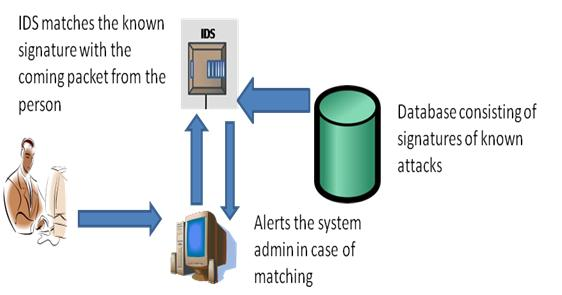
\includegraphics[width=0.7\textwidth]{Figures/Signature-based-Intrusion-Detection-System}
\decoRule
\caption[Signature based IDS]{An Signature-based intrusion detection system.}
\label{fig:Signature}
\end{figure}
\noindent Signature based methods compare so called "signatures" with an existing database of signatures. An packet or flow record is decomposed into features that together construct a signature. If the signature of an incoming flow or packet matches with a signature in the database, it is flagged as malicious. Signature-based methods have little overhead in both computation and preprocessing as it only tries to match incoming signatures to known signatures in the database. Because it only compares signatures, it is easy to deploy within a network. The system does not need to learn what the traffic within a network looks like. \\
\\
Signature based methods are very effective against known attacks. New attacks cannot be detected unless the database is updated with new signatures. It is also for attackers to avoid being caught by signature based methods, only slight modification of the "signature" is required in order to bypass the exact matching. Updating the signature database requires a lot of technical effort, since new attacks are discovered all the time.
\subsection{Anomaly based methods}
\begin{figure}[H]
\centering
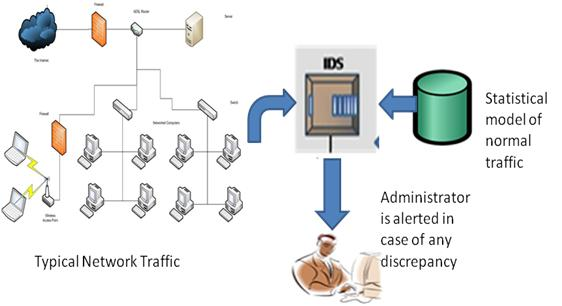
\includegraphics[width=0.7\textwidth]{Figures/Anomaly-based-Intrusion-Detection-System}
\decoRule
\caption[Anomaly based IDS]{An Anomaly-based intrusion detection system.}
\label{fig:Anomaly}
\end{figure}
\noindent Anomaly based methods, also called Behaviour based methods are methods in which the IDS tries to model the behaviour of network traffic. When an incoming packet deviates from this model, it is flagged as malicious and an alert is send. Because they use a statistical model of normal behaviour, they should be able to detect all deviations from this normal behaviour. As a result, new attacks that deviate to much from normal behaviour are detected aswell. \\
\\
Since a model of the network traffic needs to be created, the system cannot be deployed into a network and be expected to work. The system needs to learn the behaviour of the network traffic. Problems, such as generating a lot of false positive alarms, can arise when training data includes mistakes, such as misclassifications. \\
\\
Machine learning algorithms can be used as a anomaly based method. Machine learning techniques have the ability to learn from data and decide whether new data is malicous. 